\documentclass[12pt,a4paper]{article}
% math_setup.tex
% Essential Packages
\RequirePackage{etex}
\usepackage{comment}
\usepackage{etex}
\usepackage{listings}
\usepackage{amsmath}    % Advanced math typesetting
\usepackage{amsfonts}   % Math fonts
\usepackage{amssymb}    % Math symbols
\usepackage{amsthm}     % Theorem environment
\usepackage{mathtools}  % More symbols
\usepackage{tikz}       % For drawing diagrams
\usepackage{tikz-network}
\usepackage{pgfplots}
\usetikzlibrary{calc, arrows.meta, positioning, quotes}
\usepackage{mdframed}
\usepackage{float}
\usepackage{thmtools}
\usepackage{xcolor}
\usepackage{geometry}
\usepackage{fancyhdr}
\usepackage[colorlinks=true, linkcolor=blue, citecolor=green, urlcolor=red]{hyperref}
\usepackage{csquotes}
\usepackage[backend=biber, style=ieee]{biblatex}
\pgfplotsset{compat=1.18}
%\usepackage{mdframed}

% Wolfram Code Block
\lstdefinelanguage{Wolfram}{
    keywords={Sum, If, For, While, Do, Plot, Table, Range, Integrate, NIntegrate, D, Solve, NSolve, DSolve, NDSolve, LinearSolve, Expand, Factor, Simplify, FullSimplify, Module, Block, With},
    sensitive=true,
    morecomment=[l]{(*},
    morecomment=[s][\itshape]{(*}{*)},
    morestring=[b]",
    morestring=[b]',
}

\lstset{
    language=Wolfram,
    basicstyle=\ttfamily,
    keywordstyle=\color{blue}\bfseries,
    commentstyle=\color{green}\itshape,
    stringstyle=\color{red},
    showstringspaces=false,
    frame=single,
    breaklines=true,
    numbers=left,
    numberstyle=\tiny\color{gray},
    stepnumber=1,
    numbersep=5pt,
    backgroundcolor=\color{lightgray!20}
}

% add ref
\addbibresource{references.bib}
% Define colors
\definecolor{theoremcolor}{RGB}{230,230,250}  % Light purple
\definecolor{lemmacolor}{RGB}{240,248,255}    % Alice Blue
\definecolor{propcolor}{RGB}{240,255,240}     % Light green
\definecolor{corollarycolor}{RGB}{255,250,240} % Light orange
\definecolor{axiomcolor}{RGB}{255,240,245}    % Lavender blush
\definecolor{definitioncolor}{RGB}{240,255,255} % Light cyan
\definecolor{remarkcolor}{RGB}{245,245,245}   % Light gray
\definecolor{notationcolor}{RGB}{255,250,205}

% Boxed environments

\declaretheoremstyle[
    headfont=\normalfont\bfseries,
    bodyfont=\normalfont,
    headpunct={:},
    postheadspace=1em,
    mdframed={
        linecolor=black,
        backgroundcolor=definitioncolor,
        topline=true,
        bottomline=true,
        leftline=true,
        rightline=true,
        roundcorner=5pt
    }
]{boxeddefinitionstyle}

\declaretheorem[style=boxeddefinitionstyle, name=Definition]{definition}

\declaretheoremstyle[
    headfont=\normalfont\bfseries,
    bodyfont=\normalfont,
    headpunct={:},
    postheadspace=1em,
    mdframed={
        linecolor=black,
        backgroundcolor=theoremcolor,
        topline=true,
        bottomline=true,
        leftline=true,
        rightline=true,
        roundcorner=5pt
    }
]{boxedtheoremstyle}

% Theorem
\declaretheorem[style=boxedtheoremstyle, name=Theorem]{theorem}

% Lemma (adjust color)
\declaretheoremstyle[
    headfont=\normalfont\bfseries,
    bodyfont=\normalfont,
    headpunct={:},
    postheadspace=1em,
    mdframed={
        linecolor=black,
        backgroundcolor=lemmacolor,
        topline=true,
        bottomline=true,
        leftline=true,
        rightline=true,
        roundcorner=5pt
    }
]{boxedlemmastyle}
\declaretheorem[style=boxedlemmastyle, name=Lemma]{lemma}

% Proposition (adjust color)
\declaretheoremstyle[
    headfont=\normalfont\bfseries,
    bodyfont=\normalfont,
    headpunct={:},
    postheadspace=1em,
    mdframed={
        linecolor=black,
        backgroundcolor=propcolor,
        topline=true,
        bottomline=true,
        leftline=true,
        rightline=true,
        roundcorner=5pt
    }
]{boxedpropstyle}
\declaretheorem[style=boxedpropstyle, name=Proposition]{proposition}

% Corollary (adjust color)
\declaretheoremstyle[
    headfont=\normalfont\bfseries,
    bodyfont=\normalfont,
    headpunct={:},
    postheadspace=1em,
    mdframed={
        linecolor=black,
        backgroundcolor=corollarycolor,
        topline=true,
        bottomline=true,
        leftline=true,
        rightline=true,
        roundcorner=5pt
    }
]{boxedcorollarystyle}
\declaretheorem[style=boxedcorollarystyle, name=Corollary]{corollary}

% Axiom (boxed)
\declaretheoremstyle[
    headfont=\normalfont\bfseries,
    bodyfont=\normalfont,
    headpunct={:},
    postheadspace=1em,
    mdframed={
        linecolor=black,
        backgroundcolor=axiomcolor,
        topline=true,
        bottomline=true,
        leftline=true,
        rightline=true,
        roundcorner=5pt
    }
]{boxedaxiomstyle}
\declaretheorem[style=boxedaxiomstyle, name=Axiom]{axiom}

% Remark environment
\declaretheoremstyle[
    headfont=\normalfont\bfseries,
    bodyfont=\normalfont,
    headpunct={:},
    postheadspace=1em,
    mdframed={
        linecolor=black,
        backgroundcolor=remarkcolor,
        topline=true,
        bottomline=true,
        leftline=true,
        rightline=true,
        roundcorner=5pt
    }
]{remarkstyle}
\declaretheorem[style=remarkstyle, name=Remark, numbered=no]{remark}
% Normal, non-italic environments
\declaretheoremstyle[
    headfont=\normalfont\bfseries,
    bodyfont=\normalfont,
    headpunct={:},
    postheadspace=1em,
]{normalstyle}

% Notation environment
\declaretheoremstyle[
    headfont=\normalfont\bfseries,
    bodyfont=\normalfont,
    headpunct={:},
    postheadspace=1em,
    mdframed={
        linecolor=black,
        backgroundcolor=notationcolor,
        topline=true,
        bottomline=true,
        leftline=true,
        rightline=true,
        roundcorner=5pt
    }
]{boxednotationstyle}
\declaretheorem[style=boxednotationstyle, name=Notation]{notation}


% Note environment (more noticeable, with separators, no background, no end symbol)
\newenvironment{note}[1][]
    {\par\vspace{0.5em}\noindent\rule{\textwidth}{0.4pt}\par\vspace{0.5em}%
    \textbf{Note\if\relax\detokenize{#1}\relax\else: #1\fi}\par}
    {\par\vspace{0.5em}\noindent\rule{\textwidth}{0.4pt}\par\vspace{0.5em}}

\declaretheorem[style=normalstyle, name=Note, numbered=no]{oldnote}

\declaretheorem[style=normalstyle, name=Example]{example}
\declaretheorem[style=normalstyle, name=Exercise]{exercise}
\declaretheorem[style=normalstyle, name=Statement]{statement}
\declaretheorem[style=normalstyle, name=Solution, numbered=no]{solution}

% Proof environment (normal, non-italic, with QED symbol)
\declaretheoremstyle[
    headfont=\normalfont\bfseries,
    bodyfont=\normalfont,
    headpunct={:},
    postheadspace=1em,
    qed=$\blacksquare$
]{proofstyle}

\declaretheorem[style=proofstyle, name=Proof]{customproof}

% Shorthand
\newcommand{\vect}[1]{\mathbf{#1}} % For regular vectors
\newcommand{\uvec}[1]{\hat{\mathbf{#1}}} % For unit vectors
\newcommand{\prob}[1]{
    \section*{Problem #1}
}
\newcommand{\R}{\mathbb{R}} % Real numbers
\newcommand{\Z}{\mathbb{Z}} % Integers
\newcommand{\C}{\mathbb{C}} % Complex numbers
\newcommand{\N}{\mathbb{N}} % Natural numbers
\newcommand{\Q}{\mathbb{Q}} % Rational numbers
\newcommand{\Hq}{\mathbb{H}} % Quaternions
\newcommand{\F}{\mathbb{F}} % Finite fields
\newcommand{\Proj}{\mathbb{P}} % Projective space
\newcommand{\K}{\mathbb{K}} % Arbitrary field
\newcommand{\T}{\mathbb{T}} % Torus or sometimes denoted for Topological space
\newcommand{\A}{\mathbb{A}} % Affine space
\newcommand{\0}{\mathbf{0}} % Zero vector
\newcommand{\mbf}[1]{\mathbf{#1}} 
\newcommand{\mat}[1]{\mathbf{#1}}
\newcommand{\adj}{\operatorname{adj}}
\newcommand{\dom}[1]{
    \operatorname{dom}(#1)
}




% Layout
\geometry{a4paper, margin=1in}
\pagestyle{fancy}
\fancyhf{}
\rhead{\today}
\lhead{\textbf{ENG1005 Engineering Mathematics}}
\rfoot{Page \thepage}


\begin{document}

\title{ENG1005 Week5 Workshop Problem Set Solutions}
\author{Yang Xingyu (33533563)}
\date{\today}
\maketitle

\section*{Problem 1}
\begin{solution}
To show that $T=kl^2$ for some constant $k$ and $l$ as the distance variable, we need to further interpret the information given in mathematical and formal language.

Firstly, we know that $P$ is proportionate to $\frac{1}{r^2}$, or rather, when $\frac{1}{r^2}$ is fixed, we can find a linear relation between $P$ and $\frac{1}{r^2}$, that is
\[
P \propto \frac{1}{r^2} \implies \exists k_1 \in \R, \forall r\in \R_{> 0}, P = \frac{k_1}{r^2}.
\]

This allows us to define a mapping $P: \R \to \R$ that $P(r) := \frac{k_1}{r^2}$, where $k_1$ is some constant.

Secondly, from that
\begin{quote}
\textit{The power consumption $T$ of the access point is directly proportional to its output signal power $P$ measured 1 meter away.}
\end{quote}
Similarly, we have 
\[
T \propto P(1) \implies T = k_2 P(1),
\]
where $k_2$ is another constant. 

As $k_2P(1)$ is closed in $\R$, we can deduce that $T$ can be treated as a constant function under a mapping $T: S \to \R$, where $S$ is any non-empty set (we can pick which ever helpful for problem solving) such that $T(s) := k_2P(1)$.

Now we will show that in general, the power consumption of the access point with a user $l$ metres away is $T = kl^2$
for some constant $k$.

From 
\begin{quote}
\textit{The new WiFi access point will negotiate its signal power with the receiver so that the signal
received by the receiver is always the same strength no matter how far away they are.}
\end{quote}
So we have $P(l) = \frac{k_1}{l^2}$, $k_1 = P(l)l^2$, where $P(l)$ is some constant in $\R$. By definition of $P$ and $T$, $T = k_2\frac{k_1}{1^2}$, when $r=1$. Since $k_1 = P(l)l^2$, 
\[
T = k_2\frac{P(l)l^2}{1^2} = k_2P(l)l^2.
\]

Combining all constants to $k$, we have
\[
T = kl^2,
\]
where $l$ is the distance between the user and access point.
\end{solution}

\section*{Problem 2}
\begin{solution}
    To get the constant $k$, we simply solve $0.5= 5^{2}k$, and $k = \frac{1}{50}$.
\end{solution}

\section*{Problem 3}
\begin{solution}
Using information provided, we set up a Cartesian coordinate with the receiver in Abby's bedroom as origin, and define the horizontal axis $x$-axis, and the vertical axis $y$-axis.

\begin{figure}[H]
    \centering
    \begin{tikzpicture}
    % Define the axes
    \draw[->] (0,0) -- (5,0) node[right] {$x$};
    \draw[->] (0,0) -- (0,4) node[above] {$y$};
    
    
    % Mark points
    \fill[red] (0,0) circle (2pt) node[above right] {A(0,0)};
    \fill[blue] (15/18*5,0) circle (2pt) node[below left] {C(15,0)};
    \fill[green] (0,10/18*5) circle (2pt) node[below right] {B(0,10)};
\end{tikzpicture}
\end{figure}
\end{solution}

\section*{Problem 4}
\begin{solution}
    Assume that the access point is placed in $P(x,y)$, we can get the direction vector between each receiver and the access point.
    \[
    \begin{cases}
        \overrightarrow{PA} = (x,y)\\
        \overrightarrow{PB} = (x, y-10)\\
        \overrightarrow{PC} = (x-15,y)
    \end{cases}
    \]

    Taking modulus, we have 
    \[
    \begin{cases}
        |\overrightarrow{PA}| = \sqrt{x^{2} +y^{2}}\\
        |\overrightarrow{PB}| = \sqrt{x^{2} +( y-10)^{2}}\\
        |\overrightarrow{PC}| = \sqrt{(x-15)^{2} +y^{2}}
    \end{cases}
    \]

Substitute each of these into $T(l) = 0.02l^2$, we have the power consumption for each receiver
\[
\begin{cases}
    T_a = 0.02(x^{2} +y^{2})\\
    T_b = 0.02(x^{2} +( y-10)^{2})\\
    T_c = 0.02((x-15)^{2} +y^{2})
\end{cases}.
\]

It is assumed in the problem that the total power consumption is obtained by summing up consumption of each receiver requires. Addition of real functions in closed in $\R^\R$, thus we can define the function of total power consumption $T: \R \to \R$,
\[
T(x,y) = T_a + T_b + T_c =0.02\left(3x^{2} +3y^{2} -30x-20y+325\right).
\]  
\end{solution}

\section*{Problem 5}
\begin{comment}
\begin{figure}[H]
    \centering
    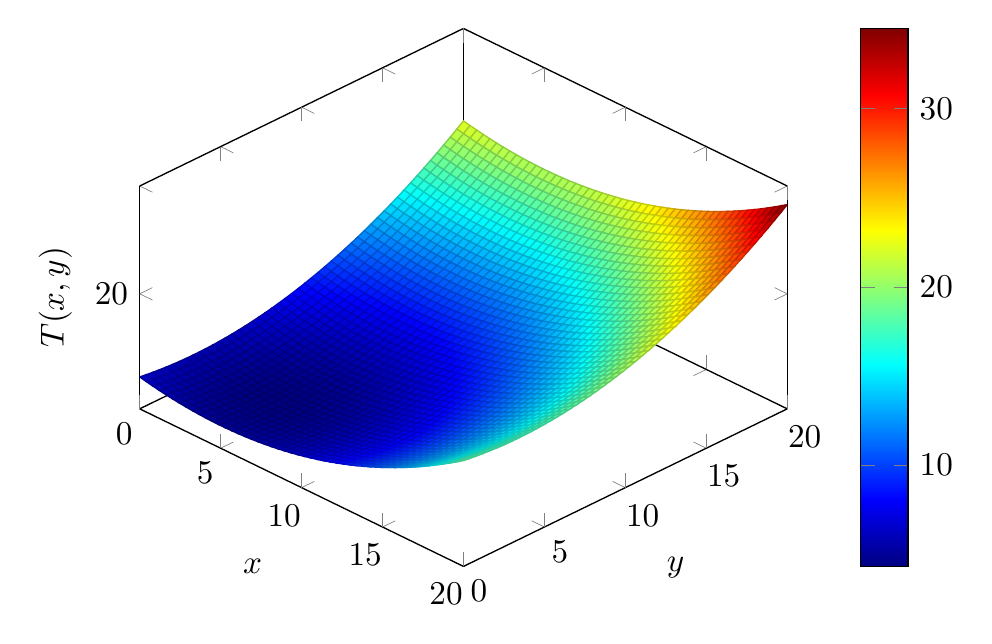
\begin{tikzpicture}[scale=1.2]
    \begin{axis}[
        view={45}{45}, % Slightly higher and different angle for better visibility
        xlabel={$x$},
        ylabel={$y$},
        zlabel={$T(x,y)$},
        colormap/jet, % Choose a color map
        colorbar, % Add colorbar
        colorbar style={ylabel={}}, % Label for the colorbar
        samples=50, % Start with moderate sample size
        ]
        \addplot3[
            surf, % Generate a surface plot
            domain = 0:20,
            y domain = 0:20,
        ]
        {0.02*(3*x^2 + 3*y^2 - 30*x - 20*y + 325)};
    \end{axis}
    \end{tikzpicture}
    \caption{$T(x,y)$}
\end{figure}
\end{comment}

\begin{figure}[H]
    \centering
    \begin{tikzpicture}[scale=1.2]
    \begin{axis}[
        view={0}{90}, % Set the view angle
        xlabel={$x$},
        ylabel={$y$},
        zlabel={$T(x,y)$},
        colormap/jet, % Choose a color map
        samples=50,
        domain=0:20,
        y domain=0:20,
        ]
        \addplot3[
            contour gnuplot={
                levels={0,5,10,15,20,25}, % Specify contour levels
                labels=true, % Add labels to contours
            },
            thick,
        ]
        {0.02*(3*x^2 + 3*y^2 - 30*x - 20*y + 325)};
    \end{axis}
    \end{tikzpicture}
    \caption{Contours of $T(x,y)$ (overhead view)}
\end{figure}

\begin{comment}
\begin{figure}[H]
    \centering
    \begin{tikzpicture}[scale=1.2]
    \begin{axis}[
        view={45}{45}, % Set the view angle
        xlabel={$x$},
        ylabel={$y$},
        zlabel={$T(x,y)$},
        colormap/jet, % Choose a color map
        samples=50,
        domain=0:20,
        y domain=0:20,
        ]
        \addplot3[
            contour gnuplot={
                levels={0,5,10,15,20,25}, % Specify contour levels
                labels=true, % Add labels to contours
            },
            thick,
        ]
        {0.02*(3*x^2 + 3*y^2 - 30*x - 20*y + 325)};
    \end{axis}
    \end{tikzpicture}
    \caption{Contours of $T(x,y)$ (oblique view)}
\end{figure}
\end{comment}

\section*{Problem 6}
\begin{solution}
    The gradient vector of $T$, is
    $\nabla T = \left(\frac{\partial T}{\partial x}, \frac{\partial T}{\partial y}\right)$.

We now find partial derivative with respect to each variable.
\begin{align*}
    \frac{\partial T}{\partial x} &= 0.02 \times \frac{\partial \left(3x^{2} + 3y^{2} - 30x - 20y + 325\right)}{\partial x} \\
    &= 0.02 \times \left(\frac{\partial (3x^{2})}{\partial x} + \frac{\partial (3y^{2})}{\partial x} - \frac{\partial (30x)}{\partial x} - \frac{\partial (20y)}{\partial x} + \frac{\partial (325)}{\partial x}\right) \\
    &= 0.02 \times \left(6x + 0 - 30 - 0 + 0\right) \\
    &= 0.02 \times \left(6x - 30\right) \\
    &= 0.02 \times 6(x - 5) \\
    &= 0.12(x - 5)
\end{align*}

\begin{align*}
    \frac{\partial T}{\partial y} &= 0.02 \times \frac{\partial \left(3x^{2} + 3y^{2} - 30x - 20y + 325\right)}{\partial y} \\
    &= 0.02 \times \left(\frac{\partial (3x^{2})}{\partial y} + \frac{\partial (3y^{2})}{\partial y} - \frac{\partial (30x)}{\partial y} - \frac{\partial (20y)}{\partial y} + \frac{\partial (325)}{\partial y}\right) \\
    &= 0.02 \times \left(0 + 6y - 0 - 20 + 0\right) \\
    &= 0.02 \times \left(6y - 20\right) \\
    &= 0.02 \times 6(y - \frac{10}{3}) \\
    &= 0.12(y - \frac{10}{3})
\end{align*}

Hence, the gradient vector is $\nabla T = \left(0.12(x - 5), 0.12(y - \frac{10}{3})\right)$.
\end{solution}

\section*{Problem 7}
\begin{solution}
From the access point is at the centre of the house, we can locate the position vector of the access point $P=(7.5, 5)$. To identify whether increase or decrease, we need to find a unit vector on $PA$'s direction, that is
\[
\widehat{PA} = \frac{\overrightarrow{PA}}{|PA|} = \frac{\left(-7.5, -5.0 \right)}{\sqrt{81.25}} = \left(-\frac{7.5}{\sqrt{81.25}},-\frac{5}{\sqrt{81.25}}\right)
\]

Now we examine the directional derivative of $T(x,y)$ along $\widehat{PA}$.
\[
D_{PA}T(7.5,5) = \nabla T(7.5,5) \cdot \widehat{PA} = (0.3, 0.2) \cdot \left(-\frac{7.5}{\sqrt{81.25}},-\frac{5}{\sqrt{81.25}}\right)
\]

Obviously, $D_{PA}T(7.5,5) < 0$, so the power consumption decreases on this direction.
\end{solution}

\section*{Problem 8}
\begin{solution}

Alternatively, the gradient derivative is defined by
\[
D_{PA}T(x,y) = \nabla T(x,y) \cdot \hat{v} = |\nabla T(x,y)| |\hat{v}| \cos{\theta} = |\nabla T(x,y)|\cos{\theta},
\]

where 
\begin{itemize}
    \item $\hat{v}$ is a unit vector in the direction of some vector $\Vec{v} \in \R^3$, 
    \item $\theta$ is the angle between the gradient vector $\nabla T$ and unit vector $\hat{v}$, and $\theta \in [0, \pi]$.
\end{itemize}

Since $|\nabla T(x,y)|$ is constant, we have
\[
\min \left(|\nabla D_{PA}T(x,y)|\right) = |\nabla T(x,y)| \min(\cos{\theta}) =
|\nabla T(x,y)| \cos{\pi} = -|\nabla T(x,y)|.
\]

 When $\cos \theta = -1$, $\theta = \arccos({-1}) = \pi$ $(\theta \in [0,\pi])$.

 Hence, when the power consumption reduces most rapidly, the access point move along the \textbf{opposite direction} to the gradient vector.
\end{solution}

\section*{Problem 9}
Now the access point is moved to the midpoint between the receivers in Abby and Ben’s rooms, that is, $Q=(0, 5)$.

We first calculate the gradient vector at $(0,5)$.
\[
\nabla T(0,5) = \left(0.12\times(-5), 0.12\times (5-\frac{10}{3})\right) = \left(-\frac{3}{5}, \frac{1}{5}\right).
\]

By conclusion from the last problem, the the greatest decrease is on the opposite direction of gradient vector. So the direction that power consumption most rapidly is 
$$-\nabla T = \left(\frac{3}{5}, -\frac{1}{5}\right)$$. 

Thus the unit vector is 
$$\frac{\left(\frac{3}{5}, -\frac{1}{5}\right)}{\sqrt{(\frac{3}{5})^2 + (-\frac{1}{5})^2}} = \left(\frac{3}{\sqrt{10}},-\frac{1}{\sqrt{10}}\right)$$.

\section*{Problem 10}
\begin{solution}
To find the most efficient position for the WiFi access point, we need to analyze the gradient of the power consumption function. The gradient vector, made up of the first-order partial derivatives, points in the direction of the steepest increase in power consumption. Minimizing power consumption involves moving the access point in the opposite direction of the gradient.

Let \( T(x, y) \) represent the power consumption as a function of the access point’s coordinates \((x, y)\). A necessary condition for \( T(x, y) \) to reach a minimum is that all components of the gradient vector are zero:

\[
\frac{\partial T}{\partial x} = 0, \quad \frac{\partial T}{\partial y} = 0
\]

When this condition is met, the gradient vector \( \nabla T(x, y) \) is the zero vector:

\[
\nabla T(x, y) = \left( \frac{\partial T}{\partial x}, \frac{\partial T}{\partial y} \right) = \mathbf{0}
\]

This indicates that there is no further decrease in power consumption in any direction, meaning the point is a critical point.

If \( T(x, y) \) is a convex function, this condition is not only necessary but also sufficient for a global minimum. For a convex function, any local minimum is also a global minimum. Thus, when the gradient is zero and convexity is confirmed, the point is the most power-efficient position. \textbf{We have shown that $T(x,y)$ is convex in the remark}.

So, at the most power-efficient location for the access point, the gradient of the power consumption function will be $\0$, indicating that power consumption cannot be further reduced.


Additionally, the existence of a zero gradient vector can be understood through the Mean Value Theorem, which guarantees that under certain conditions, there exists a point where the derivative (or gradient in the multivariable case) is zero\cite{rudin_principles_1976}.

\begin{theorem}[Mean Value Theorem for Single Variable Functions]
    Let \( f: [a, b] \rightarrow \mathbb{R} \) be a function that satisfies the following conditions:
\begin{enumerate}
    \item \( f \) is continuous on the closed interval \([a, b]\).
    \item \( f \) is differentiable on the open interval \((a, b)\).
\end{enumerate}
Then, there exists at least one point \( c \in (a, b) \) such that
\[
f'(c) = \frac{f(b) - f(a)}{b - a}.
\]
\end{theorem}

This theorem indicates that the derivative at some point \( c \) is equal to the average rate of change of the function over the interval \([a, b]\). If \( f(a) = f(b) \), this simplifies to \( f'(c) = 0 \), resembling the conclusion of Rolle's Theorem.

Now, consider the multivariable case:

\begin{theorem}[Mean Value Theorem for Multivariable Functions]
    Let \( f: D \rightarrow \mathbb{R} \) be a differentiable function, where \( D \subseteq \mathbb{R}^n \) is an open set. Suppose \( \mathbf{a}, \mathbf{b} \in D \), then there exists a point \( \mathbf{c} \) on the line segment between \( \mathbf{a} \) and \( \mathbf{b} \) such that
    \[
    f(\mathbf{b}) - f(\mathbf{a}) = \nabla f(\mathbf{c}) \cdot (\mathbf{b} - \mathbf{a}),
    \]
    where \( \nabla f(\mathbf{c}) \) is the gradient vector of \( f \) at \( \mathbf{c} \).
\end{theorem}

In the context of minimising the power consumption function \( T(x, y) \), this theorem implies that the gradient vector \( \nabla T(x, y) \) will point in the direction of the steepest ascent. Therefore, moving opposite to this direction will decrease power consumption, and the process will continue until the gradient becomes zero, indicating that a minimum has been reached.

Finally, the uniqueness of the zero gradient vector is guaranteed, as \( \mathbf{0} \) is unique in any vector space, ensuring that the critical point identified is well-defined.
\end{solution}
\begin{remark}
Below is an explanation of how to extend the second-order derivative test for convexity from univariate functions to multivariable functions, a widely used method to determine whether a multivariable function is convex.

The \textit{second derivative test} is a technique used to classify critical points of a twice-differentiable function. For a function of one variable, if the first derivative \( f'(x_0) = 0 \) at a critical point \( x_0 \), the nature of this critical point can be determined by the second derivative \( f''(x_0) \). Specifically, if \( f''(x_0) > 0 \), \( x_0 \) is a local minimum; if \( f''(x_0) < 0 \), \( x_0 \) is a local maximum. If \( f''(x_0) = 0 \), the test is inconclusive, and higher-order derivatives must be examined. In the context of convexity, a function is considered convex if its second derivative is non-negative \( f''(x) \geq 0 \) across the entire domain, which implies that the function is "curved upwards" and any local minimum is also a global minimum.

This concept extends to multivariable functions through the use of the \textit{Hessian matrix}\cite{apostol_mathematical_1974}, a matrix composed of second-order partial derivatives. In multivariable functions, the function values are influenced by more variables, and convexity means the function increases in all directions from a global minimum (which is also a local minimum). Therefore, the second derivative test is crucial, but it requires computing all possible second derivatives, resulting in a \( k \times k \) Hessian matrix, where \( k \) is the number of variables.

For example, consider the function \( T(x, y) = 0.02\left(3x^{2} + 3y^{2} - 30x - 20y + 325\right) \). The Hessian matrix for this function is given by:
\[
H(x, y) = \begin{bmatrix} 
\frac{\partial^2 T}{\partial x^2} & \frac{\partial^2 T}{\partial x \partial y} \\ 
\frac{\partial^2 T}{\partial y \partial x} & \frac{\partial^2 T}{\partial y^2} 
\end{bmatrix}
= \begin{bmatrix}
0.12 & 0 \\
0 & 0.12
\end{bmatrix}.
\]
The determinant of this Hessian matrix is \( \det(H) = 0.12 \times 0.12 - 0 \times 0 = 0.0144 \), which is positive. Since the diagonal elements \( 0.12 \) are also positive, the Hessian matrix is positive definite. According to the second derivative test, this means that the function \( T(x, y) \) has a local minimum at every point in its domain.

To check for convexity, we observe that since the Hessian matrix is positive definite across the entire domain of \( T(x, y) \), the function is convex. A positive definite Hessian matrix indicates that the function curves upwards in every direction, which is the defining property of a convex function. Therefore, \( T(x, y) = 0.02\left(3x^{2} + 3y^{2} - 30x - 20y + 325\right) \) is a convex function.
\end{remark}

\section*{Problem 11}
\begin{solution}
    To solve for $(x, y)$ that the power consumption is optimised, we simply solve
    \[
    \begin{cases}
        0.12(x-5) = 0\\
        0.12(y-\frac{10}{3}) = 0
    \end{cases}.
    \]

    We have
    \[
    \begin{cases}
        x=5\\
        y=\frac{10}{3}
    \end{cases}.
    \]

    Hence, when the access point is placed at $(5, \frac{10}{3})$, the power consumption is optimised.
    
\end{solution}

\printbibliography
\end{document}